
\section{Literature Review}\label{sec:lit_ref}

During the literature research, multiple studies and papers have been examined to evaluate the state of the art for Goertzel filter implementations. There are several areas that the previous research focused on. \\
To begin with, efforts were made to optimize the Goertzel Algorithm in terms of performance and effectiveness. Various methods were proposed, including hardware acceleration using FPGA or ASIC implementations, pipeline processing, parallel processing, and parallel processing in hardware. These optimization techniques aim to expedite processing and utilize fewer resources while maintaining accurate frequency detection.

The solution proposed by Xinyi in \cite{5630500} outlines an FPGA implementation of a modified Goertzel algorithm specifically designed for Dual Tone Multi-Frequency (DTMF) signal detection. The traditional Goertzel algorithm may not be optimal for DTMF signal detection due to the presence of multiple tones. To address this limitation, the research proposes a modified Goertzel algorithm tailored for DTMF signal detection. This modified algorithm uses a comparator (to compare if component frequency equals to the pole frequency) and a counter to omit the multiply operations and two addition operations.  In terms of the accuracy and robustness of DTMF signal detection, this approach demonstrates same performance compared to traditional Goertzel algorithms, as validated through simulations using various DTMF signal samples, however it used less hardware resources.\\
\cite{6828441} introduces a novel structure of the Goertzel filter and explores its frequency characteristics and filtering abilities. 
The structure of the Goertzel filter is presented, which consists of N mutually delayed branches of the filter. These branches are subsequently multiplexed and summed to obtain the output. 
The paper provides equations that describe the operations involved in the filtering process, emphasizing the frequency domain representation of the impulse response, decimation, up-sampling, and phase shift. The proposed system is shown to eliminate the decimation property of the Goertzel filter, allowing for the use of a specified decimation factor independent of the filter's filtration characteristics.  This is beneficial in scenarios where aliasing caused by spectral leakage due to decimation needs to be avoided. The introduced structure effectively eliminates the decimation property, providing flexibility in choosing the decimation factor.  
\begin{figure}
    \centering
    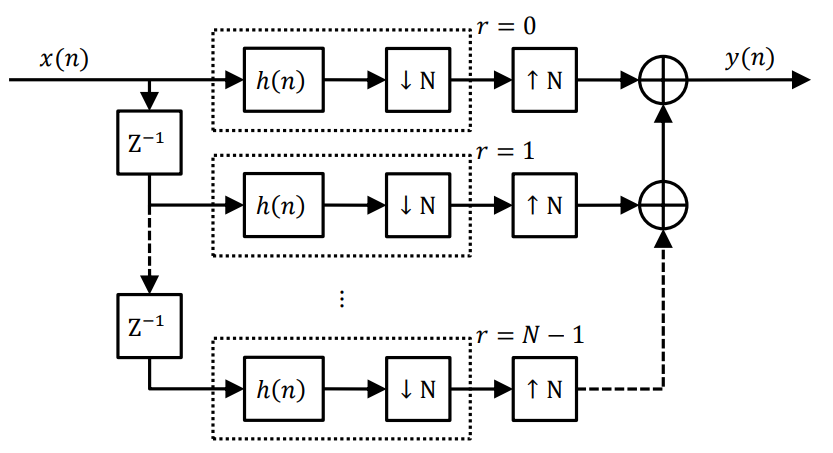
\includegraphics[width=1\linewidth]{Capture1.PNG}
    \caption{Signal diagram of the Goertzel filter in parallel in \cite{6828441}}
    \label{fig:signal_diagram_of_gf}
\end{figure}
While the structure may not always be advantageous compared to other filter structures, it can be useful in situations where a higher resolution of the signal is required temporarily, such as for synchronization purposes. \\

In \cite{958339}, Robert Beck et al. investigate the impact of coefficient quantization on the output of a second-order Goertzel filter used for signal tone detection. The authors systematically design the tone detector with minimum complexity by analyzing the effects of coefficient quantization. They identify three configurations of Goertzel filters based on different second-order digital resonators that are well-suited for VLSI implementation. These configurations exhibit complementary output sensitivities to resonator coefficient errors across the frequency range, allowing for efficient trade-offs in filter design and optimization. The authors derive analytic expressions for the tone response of a fully finite-precision Goertzel filter using the Fourier summation transform, considering both rectangular and 1/2-end-point input data window approaches. Experimental results and simulations validate the findings, demonstrating improved tone response by incorporating the derived analytic expressions into the design of a DTMF tone detector. This research offers a systematic analysis of coefficient quantization's effect on Goertzel filter performance, providing insights into the design and optimization of finite-precision Goertzel filters for tone detection applications.\\

Trevor W. Fox et al. propose in \cite{1347723} the use of Goertzel digital filters for forward and inverse Modified Discrete Cosine Transform (MDCT) calculations. The Goertzel MDCT structure is obtained from the discrete-time convolution sum representing the MDCT. The authors emphasize that these new methods require fewer arithmetic operations and are less susceptible to coefficient quantization errors compared to earlier recursive methods for MDCT. These suggested methods are particularly suitable for cost-effective fixed-point VLSI implementations. The study shows that the fixed-point versions of these algorithms significantly reduce hardware required compared to previous implementations.

The authors of \cite{6912785} specifically focus on comparing the accuracy of the Goertzel Algorithm with different precisions of fixed-point arithmetic. They conduct the algorithm using fixed-point widths ranging from 6 to 16 bits and evaluate its performance using three test signals: a single noise-free tone for accuracy assessment, noise-free multi-tones for separation quality assessment, and a single tone with additional noise for resilience assessment. The research concludes that the most accurate fixed-point arithmetic is achieved with a 16-bit precision. It is also worth-noting that using floating-point arithmetic is not viable if the CPU lacks sufficient processing power to keep up with the data. Additionally, the enhanced accuracy-speed factor of 8-bit fixed-point arithmetic cannot compensate for its extremely low frequency resolution.
\begin{figure}
    \centering
    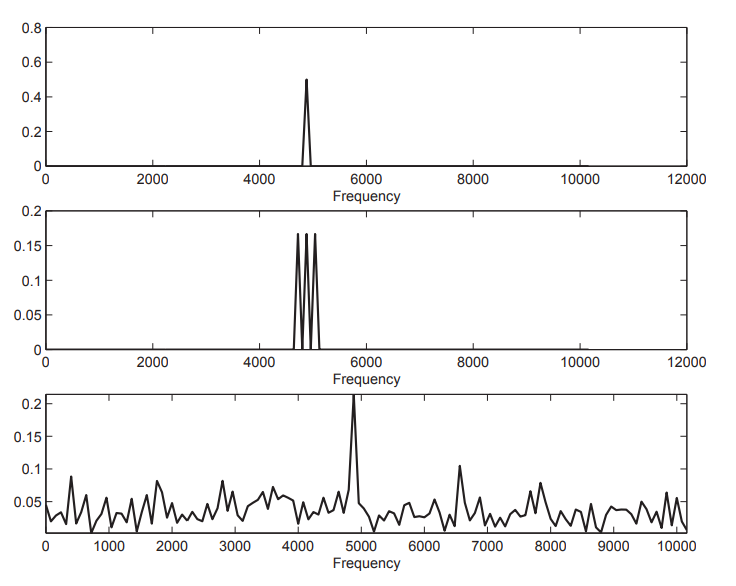
\includegraphics[width=0.75\linewidth]{img/image_2023-06-28_171752016.png}
    \caption{ FFT of the Test Signals used in \cite{6912785}}
    \label{fig:fixed_point_arithmetic_test_signals}
\end{figure}

To prevent overflows in fixed-point implementations of second-order Goertzel filters, a non-uniform or conservative scaling factor can be employed. The approach suggested in \cite{6272009} involves using a scaling factor operating in $O(1/N)$ (specifically chosen as  \(\pi/4N\)), where N represents the number of samples. This approach is based on a novel overflow analysis considering complex-valued input sequences. The study demonstrates that the second-order version, which requires fewer hardware resources, is preferable when constructing a bank of Goertzel filters. However, the reduced scaling factor necessary to prevent overflows in fixed-point arithmetic can render the aforementioned benefit obsolete. A smaller scaling factor may lower the accuracy of calculated Fourier coefficients or increase the required hardware to maintain accuracy. The authors validate their approach through experiments and compare the performance of the proposed scaling factor technique with traditional fixed-point Goertzel implementations. Various metrics, such as signal-to-noise ratio (SNR) and dynamic range, are evaluated to assess the scaling factor's effectiveness in improving filter accuracy. The results indicate that incorporating the scaling factor into the fixed-point implementation of the second-order Goertzel filter leads to improved performance, reduced quantization noise, and enhanced numerical precision. The analysis demonstrates that the scaling factor approach achieves a better trade-off between accuracy and computational efficiency compared to conventional fixed-point implementations.